\chapter{OpenCL heterogenous programming platform}
\label{chap:cl}
This chapter will describe OpenCL. A framework for writing applications that
harness computational capabilities of heterogeneous hardware environment on
which applications are run. Since the introduction of programmable pipeline
in GPUs\footnote{Graphics Processing Unit} an opportunity appeared to use
capabilities of these devices to offload highly parallel, computationally
intensive tasks from the main CPU\footnote{Central Processing Unit}. OpenCL
isn't however limited to GPUs. Multi--core processors can also be used through
its runtime without manual thread management.

OpenCL is used in programming project of this thesis described in \autoref{chap:project}.
Metaballs and Marching Cubes algorithm are implemented with it. Marching Cubes
algorithm and its OpenCL implementation are described in detail in
\autoref{chap:marchingcubes}.

\section{Introduction}
This section is based on \cite{Kirk:2010:PMP:1841511} and
\cite{gaster2012heterogeneous}.

\subsection{Beginnings of programmable GPUs}

From early 1980s to late 1990s most graphic hardware was fixed--function.
Dedicated graphics units exposed predefined, fixed set of functions that were
implemented in hardware or drivers. It wasn't possible to write custom program
that would be executed on the GPU.

As the complexity of fixed--function APIs expanded, hardware vendors implemented
them with general purpose processors that could run some limited instruction set
on many execution units. This instruction set was used to implement graphics APIs
like OpenGL or DirectX.

In 2001 NVIDIA released GeForce 3 graphics card that exposed this internal
instruction set to users of OpenGL and DirectX APIs. ATI technologies followed
with Radeon 9700 that could also run programs supplied by the user on the GPU.
DirectX 8 and OpenGL introduced programmable vertex stage. With
DirectX 9 another programmable stage was introduced, the \emph{pixel shader}\footnote{or \emph{fragment program} in
OpenGL terminology}. At this point, vertex and pixel shaders were
implemented via separate chips in the GPU. In 2005, with release of XBox 360
first unified architecture was introduced, on which vertex and fragment shaders
were run on the same processor.

Graphics processing, that these devices were build for, is very well suited for
parallelization. Vertex shader stage takes list of vertices as its input and
maps them onto the screen optionally defining colour of the vertex. Each
vertex is processed independently making it possible to process many vertices
at the same time.

Pixel shader stage receives position of the point and returns final colour of
the pixel. This also is done independently for each pixel.

\subsubsection[Early attempts at GPGPU]{Early attempts at GPGPU\footnote{General Purpose GPU}}

With the unification of computational resources in the GPUs they started to
resemble highly parallel computers. Researchers noted this fact, and tried to
harness enormous parallel performance of these devices for workloads other than
graphics.

GPUs of DirectX 9 era were still designed in graphics processing in mind.
Although there were programmable stages in the pipeline, types of input and
output parameters in each stage were severely limited. Moreover, the final
result was generated as a pixel buffer, so the programmer had to map outputs of
his algorithm to 2D screen space with pixel colour as output. Inputs to the
pixel shader stage had to be supplied by textures.

Even with these issues, researchers who managed to port their algorithms to
GPUs reported great performance benefits \parencite{gpugems2ch46}.

\subsubsection{CUDA}

When working on Tesla GPU architecture, engineers at NVIDIA realized the
potential in providing device's resources in easier way. Additional instructions
and functionalities were added to the device. Among them, read and write
operation with arbitrary offsets\footnote{Shaders could only write to predestined
places in memory, reserved for pixel output}, synchronization barriers for
groups of threads, atomic read/write operations. New parallel programming model
was developed that defined hierarchy of threads.

To expose all these features to programmers new C--like language was
created and named CUDA\footnote{Compute Unified Device Architecture}.

CUDA is capable of operating without any DirectX or OpenGL context. Device it's
run on doesn't even have to be connected to any display output. CUDA programs
are usually inlined in larger C or C++ programs and are called \emph{kernels}.
Special compiler called \emph{nvcc} is used to compile kernel code. For more
information about CUDA refer to official CUDA website\footnote{\url{http://www.nvidia.com/object/cuda_home_new.html}}.

\subsubsection{Inception of OpenCL}

On June 16th, 2008 Khronos Group announced formation of Compute Working Group (CWG)
that was tasked with establishing open standard for programming heterogeneous
CPU and GPU environments\footnote{\url{https://www.khronos.org/news/press/khronos\_launches\_heterogeneous\_computing\_initiative}}.
CWG consisted of many hardware and software vendors interested in
standardization of such API.

Compute Working Group adopted proposal of Apple Inc. that submitted programming
interface called Open Compute Language (OpenCL). Apple was already developing
OpenCL for quite some time to have it ready for its upcoming Mac OS X Snow
Leopard release.

On December 9th, 2008 final specification of OpenCL 1.0 was
released\footnote{\url{https://www.khronos.org/news/press/the\_khronos\_group\_releases\_opencl\_1.0\_specification}}.
Releases of conforming implementations from hardware vendors followed\footnote{\url{http://www.khronos.org/conformance/adopters/conformant-products/\#opencl}}.

\subsection{Specification}
OpenCL specification is maintained by the Khronos Group. It consists of C API
and Kernel language that is similar to C99. Khronos also releases official C++
wrapper API\footnote{This wrapper API is used in programming project of this thesis}.

Unofficial bindings for various languages and frameworks also exist. Among others
\begin{itemize}
	\item PyOpencl\footnote{\url{http://mathema.tician.de/software/pyopencl}}
		for Python
	\item JOCL\footnote{\url{http://www.jocl.org/}} for Java.
	\item fortrancl\footnote{\url{http://code.google.com/p/fortrancl/}} for Fortran
	\item gocl\footnote{\url{https://github.com/elima/gocl}} wrapper for C
		applications based on GObject
	\item QtOpenCL\footnote{\url{http://doc.qt.digia.com/opencl-snapshot/index.html}}
		wrapper based on Qt library semantics.
\end{itemize}

\section{Logical abstraction of computational resources}
\label{sec:cllogicalabstraction}
OpenCL aims to be API that lets hardware manufacturers expose various kinds of
devices to the programmers in a consistent and abstracted way. To fulfil this
requirement OpenGL defines logical hierarchy of computational resources.
Hardware vendors map real hardware to this abstraction in their implementations
of OpenCL.

OpenCL defines one processor (\emph{host}) that is coordinating execution of
OpenCL kernels on one or more \emph{devices}. Host, is executing functions from
C API portion of the specification. It's responsible for discovering available
devices, setting up contexts for them, allocating memory on host and devices,
queuing execution of kernels and initiating transfer of data between various
memories.

Diagram of this logical structure is presented in \autoref{fig:clhw}.

\subsection{Platforms}

On the top of the hierarchy there is a \emph{Platform}. It is usually an implementation
of OpenCL by a single vendor. To query list of available platform in the system
function \texttt{clGetPlatformIds()} must be called twice. Once with parameter
\texttt{platforms} set to \texttt{NULL} to obtain number of platforms, and
second time, with \texttt{platform} parameter set to array that will fit
number of \texttt{cl\_platform\_id} structures equal or greater than the number
in argument \texttt{num\_platforms} retrieved on first invocation of this
function\footnote{This pattern should be used for discovering other types of resources
in OpenCL as well}.

Note however, that OpenCL is usually loaded as a dynamic library provided by
vendor. These libraries will usually return only one platform.

To address this problem Khronos Group introduced \texttt{cl\_khr\_icd} extension
that will look for list of installed OpenCL
ICDs or Installable Client Drivers in place specific for given OS. If
implementation supports this extension, new function \texttt{clIcd\-Get\-Platform\-IDsKHR}
is available that will present to the user platforms from all vendors available
on the system. This extension also makes sure, that function calls with OpenCL
object created in certain platform will be routed to implementations in this
platform.

\begin{figure}[hb]
	\begin{center}
		%\includegraphics[scale=0.7]{chapters/opencl/opencl_hwmodel.jpg
	  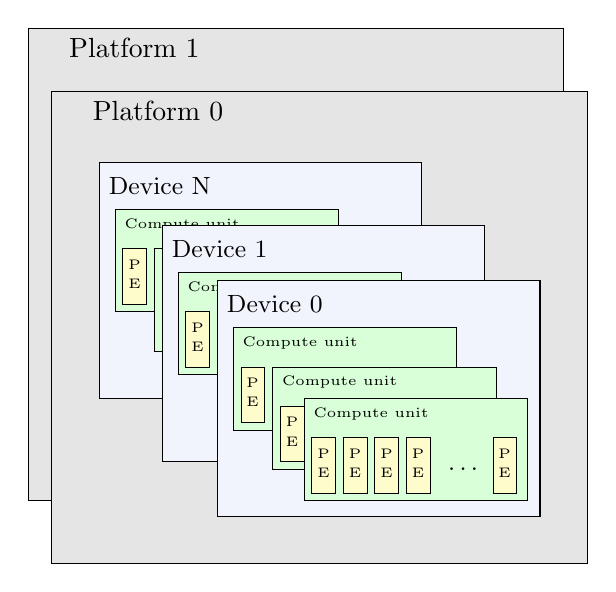
\begin{tikzpicture}

\draw[fill=gray!20] (0.3,-2) rectangle ++(6.8,6) node[anchor=north east] at ++(-4.5,0) {Platform 1};

\draw[fill=gray!20] (0.6,-2.8) rectangle ++(6.8,6) node[anchor=north east] at ++(-4.5,0) {Platform 0};

\foreach \x/\xtext in {1/N,1.8/1,2.5/0}
{
  \draw[fill=blue!85!green!5] (\x+0.2,3.3-\x) rectangle ++(4.1,-3);
  \draw[font=\small] node[anchor=west] at (\x+0.2, 3-\x){Device \xtext};
  \foreach \y in {0.5,1,1.4}
  {
    \draw[very thin,fill=green!15, opacity=10] (\x+\y-0.1, 3.2-\x-\y) rectangle ++ (2.84,-1.3);
    \node[font=\tiny,anchor=north west] at (\x+\y-0.1, 3.2-\x-\y) {Compute unit};
    \foreach \z in {0.1, 0.5, 0.9,1.3, 2.4}
   {
     \draw[very thin,fill=yellow!20] (\x+\y-0.1 + \z, 2.7-\x-\y) rectangle ++(0.3, -0.7);
     \draw[font=\tiny] node at ( (\x+\y + \z + 0.05, 2.5-\x-\y) {P};
     \draw[font=\tiny] node at ( (\x+\y + \z + 0.05, 2.25-\x-\y) {E};
   }
   \draw[font=\small] node at  ( (\x+\y + 1.95, 2.3-\x-\y) {\ldots};
  }
}
\end{tikzpicture}
	\end{center}
	\caption{Logical partitioning of hardware in OpenCL}
	\label{fig:clhw}
\end{figure}

\subsection{Devices}

Platform, may contain one or more \emph{devices}. Devices are units that
actually execute the kernel code. Device may map for example to single GPU or
CPU.

For example, NVIDIA OpenCL implementation presents each GPU available in the
system as separate device. OpenCL from AMD besides presenting GPUs also presents
supported CPUs as devices.

Device is last entity in hierarchy that has its distinct API object. Further
elements cannot be operated on, and are just abstract concepts to which vendors
map their hardware.

These elements are \emph{compute units} which are comprised of \emph{processing
elements}. Devices can be queried for number of compute units they contain
through \texttt{clGetDeviceInfo()} function.


Exact details of mapping is dependant on OpenCL vendor. Underlying architectures
of GPUs, CPUs and DSPs\footnote{Digital Singal Processors} can differ greatly
even within the same class of devices.

Specifics of implementation on selected devices supporting OpenCL will be
presented in \autoref{sec:climpl}.

\section{Memory model}

OpenCL provides layer of abstraction on device memory. Depending on the
capabilities of given device, some of memories described below may be
unavailable.

Below are descriptions of memories defined by OpenCL specification. They are
divided to Host--side and Device--side memories.


\subsection{Host--side memory model}

This is the model from the perspective of code that runs on the host. The one
that executes OpenCL library functions. Three types of memory are distinguishable
in this context:

\begin{description}
  \item[Host memory] \hfill \\
    Memory allocated by the host code with standard allocation techniques
    like \texttt{malloc()}. It's not managed by the OpenCL runtime.
  \item[Buffers] \hfill \\
    Objects that are handles for global or constant memory allocated on host.
    Buffers are similar in nature to flat C arrays. They have linear addressing,
    so pointer arithmetic is possible in kernel code.

    Buffers differ however in one one crucial point with host memory. Operations
    on them are asynchronous. Functions like \texttt{clEnqueue\-Read\-Buffer()} that
    transfer data between host and device return immediately, and the transfer
    starts in the background. Event mechanism may be used for synchronization
    (see \autoref{sub:clevents}).
  \item[Images] \hfill \\
    Images are somewhat similar to buffers, but differ in several ways.
    Unlike buffers, images can be multidimensional. They are not laid flatly in
    memory, but in a way that preserves spatial locality of points within the
    image\footnote{For example by Z--order mapping \parencite[p. 111-113]{gaster2012heterogeneous}},
    so they cannot be adressed directly but through sampling object, that define
    access patterns to images. They are also limited in terms of supported
    datatypes to ones that are relevant in graphics; no arbitrary structures can
    be held in images.

    Images are abstraction of texturing units available in GPU shaders. Because
    of this heritage, images are not supported by every OpenCL implementation.

\end{description}
\begin{figure}[ht]
  \begin{center}
    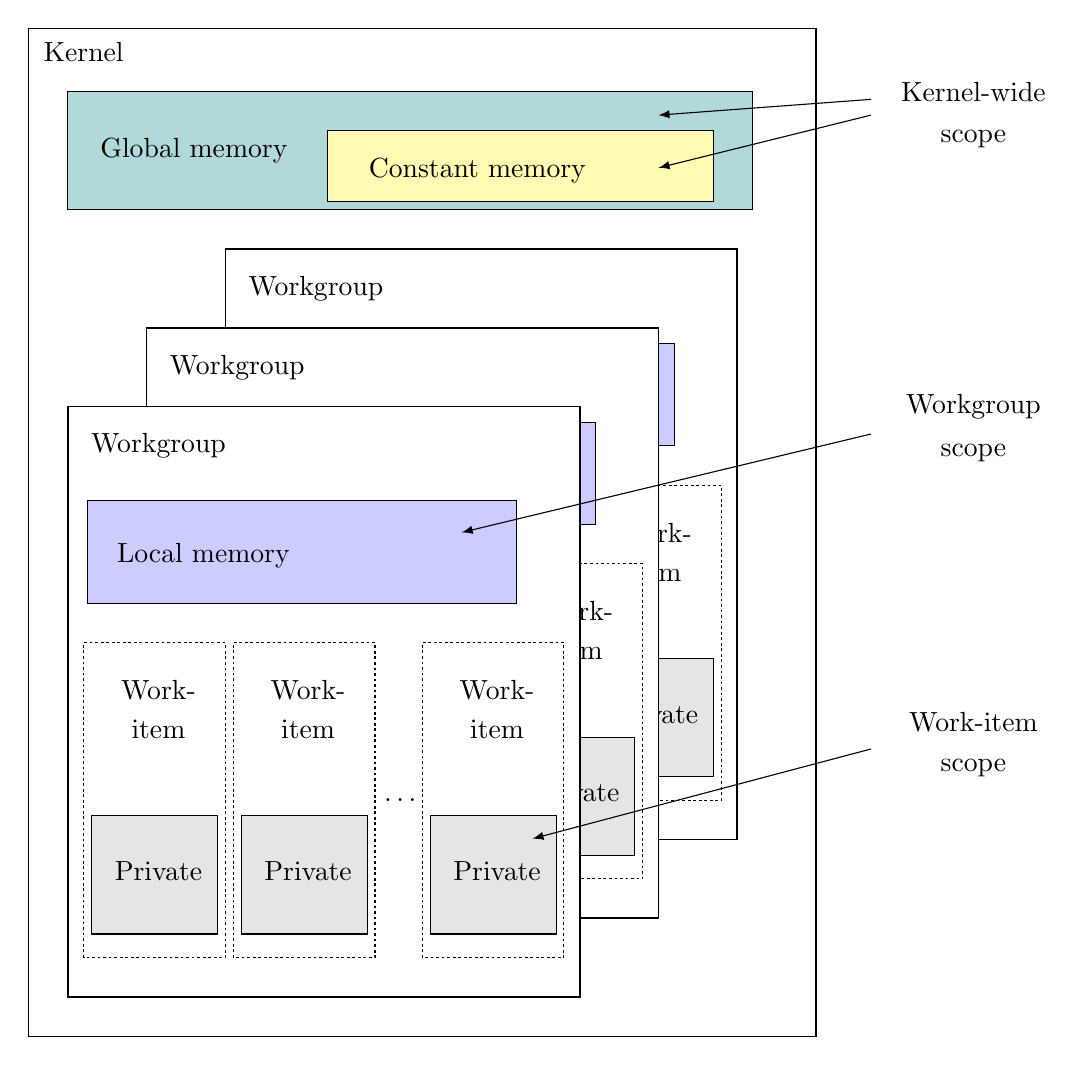
\begin{tikzpicture}[]
\draw[semithick] (0,0) rectangle (10,12.8);
\draw node at (0.7,12.5) {Kernel};
\foreach \x in {3,2,1}
{
  \draw[semithick,fill=white] (\x-0.5,\x-0.5) rectangle (\x+6,\x+7);
  \draw node at (\x+0.65,\x+6.5) {Workgroup};
  \draw[thin,fill=blue!20,fill opacity=40] (\x-0.25, \x+4.5) rectangle (\x+5.2, \x+5.8);
  \draw node [anchor=west] at(\x,\x+5.1) {Local memory};
  \foreach \y in {1, 2.90, 5.3}
  {
    \draw[thin,dashed, dash pattern = on 1pt off 1pt] (\x+\y-1.3, \x) rectangle (\x+\y+0.5, \x+4);
    \draw node at (\x+\y-0.35, \x+3.4) {Work-};
    \draw node at (\x+\y-0.35, \x+2.9) {item};
    \draw[thin,fill=gray!20,fill opacity=40] (\x+\y-1.20,\x + 0.3) rectangle (\x+\y+0.4,\x+1.8);
    \draw node at (\x+\y-0.35, \x+1.1) {Private};
  }
  \draw node at (\x+3.75, \x+2) {\ldots};
}

\draw[fill=blue!50!green!30] (0.5, 10.5) rectangle (9.2,12);
\draw node at (2.1, 11.25) {Global memory};

\draw[fill=yellow!30!] (3.8, 10.6) rectangle (8.7,11.5);
\draw node at (5.7, 11) {Constant memory};

\draw node at (12, 12) {Kernel-wide};
\draw node at (12, 11.4) {scope};
\draw[-latex] (10.7,11.9) -- (8,11.7);
\draw[-latex] (10.7,11.7) -- (8,11.03);

\draw node at (12, 8) {Workgroup};
\draw node at (12, 7.4) {scope};
\draw[-latex] (10.7,7.65) -- (5.5,6.4);

\draw node at (12, 4) {Work-item};
\draw node at (12, 3.4) {scope};
\draw[-latex] (10.7,3.65) -- (6.4,2.51);
\end{tikzpicture}
  \end{center}
  \caption{Abstract memory model of OpenCL \parencite{gaster2012heterogeneous}}
  \label{fig:clmemmodel}
\end{figure}
\todo{If time allows, write about pinned memory}
\subsection{Device-side memory model}

These are OpenCL memory types, as seen from kernel perspective.

\begin{description}
  \item[Global memory] \hfill \\
    Kernel-wide memory that is visible to all compute units on the device.
    It is the only memory that can be used for transferring data between host and
    devices. This is also usually slowest type of memory on the device by raw
    throughput.
  \item[Constant memory] \hfill \\
    Memory designated for data that is going to be accessed simultaneously by
    many threads. Its contents cannot change throughout the lifetime of the
    kernel. If available it's usually implemented with specialized hardware
    and/or caching strategies.
  \item[Local memory] \hfill \\
    Special memory area that resembles software--controlled cache. This area is
    valid only within a single workgroup (see \autoref{subsub:clworkgroups}). It's
    expected to be much faster than global memory\footnote{However it's not guaranteed},
    so it can be used as a scratchpad area for threads in one workgroup.

    It may be implemented e.g. as separate chip in Compute Unit.

    Local memory can be declared for workgroup in two ways, either dynamically,
    by setting kernel parameter prefixed with \texttt{\_\_local} to NULL with
    desired size parameter, or statically as an array in kernel with the same
    prefix.

  \item[Private memory] \hfill \\
    Memory valid within a single thread. Every non-prefixed variable and all function
    arguments that are not pointers land in this memory. It may be implemented
    with registers\footnote{execution on GPUs isn't stack--based, so every variable
    is stored in very limited number of registers}. If number of registers is
    exceeded, they may be spilled to global memory, what can have very
    detrimental impact on performance. Number of registers used by kernel must
    be thus carefully controlled.

    Private memory is the fastest available type of memory. For GPUs it's usually
    orders of magnitude faster than global or local memory.
\end{description}

\section{Execution model}
\label{sec:clexecmodel}

This section will describe OpenCL object that mange execution of programs on the
device and stages of such execution.

\subsection{Context}

Context is a structure that coordinates communication between host and devices
and keeps information about memory objects. 

It is created by providing list of devices to \texttt{clCreateContext()}
function. Devices must all come from the same platform, as returned by
\texttt{clGetDeviceIDs()}. There is a convenience function \texttt{clCreate\-Contex\-FromType()}
that creates context from all devices of given type from one platform \parencite{openclspec}.

\subsection{Programs and Kernels}

To execute kernel code on the device, it must be first provided to specialized
compiler that tranlates human--readable source code to machine--specific
instructions.

Kernel code must be fed to \texttt{clCreate\-Program\-WithSource()} function in the form of
pointer to character array. OpenCL implementation takes this textual
representation and translates it in runtime. It's worth noting, that OpenCL kernel
code is provided to the library in the source form. This may be not suitable for
secret proprietary algorithms. For this reason, with OpenCL 2.0 Provisional
specification, Khronos released definition of common intermediate
representation called SPIR\footnote{Standard Portable Intermediate Representation
  \url{http://www.khronos.org/registry/cl/specs/spir_spec-1.2-provisional.pdf}}.

There is another function that creates program objects named\\
\texttt{clCreate\-Program\-With\-Binary()}. It takes binary representation of OpenCL
code. This function however, is highly device--specific. It can only be used
for caching compiled programs the first time application is run so no compilation
is needed during subsequent runs.

After creating program object, it isn't yet compiled. Compilation is triggered
by \texttt{cl\-Build\-Program()} function.

One program object may have been compiled from a source string containing many
OpenCL kernels. Each function prefixed with \texttt{\_\_kernel} in such string
may be used to create separate kernel with \texttt{clCreate\-Kernel()} function by
providing build program object and kernel function name, or with
\texttt{clCreateKernelsInProgram()} function that creates kernel objects from
all kernel functions present in program object.

\subsubsection{Supplying arguments to kernels}

Since kernels aren't normal host function, they aren't invoked as such. Because
of that, arguments for kernels must be supplied in specific way. Each argument
must be set with separate call to function \texttt{clSetKernelArg()}. This style
of argument settings resembles the way arguments are supplied to shaders in OpenGL
or DirectX.

\subsection{Command queues}

With kernel arguments properly set up, it can be queued for execution on the
device with \texttt{clEnqueueNDRangeKernel()}\footnote{Enqueue N-dimensional range kernel}
function. Kernels are scheduled for execution on \emph{command queues} --- special
objects that are tied to particular device and are used for management of tasks
on this device.

There may be many command queues created with single
device\footnote{For e.g. multiple application threads}. Conformant OpenCL
implementation guarantees, that as long as these command queues don't use the
same resources, like memories, programs and kernels, at the same time, no
synchronization is needed. Otherwise, special care must be taken to ensure
consistency. Using shared objects on many queues is described in Appendix A
of the OpenCL specification \parencite{openclspec}.

\subsubsection{Workgroups and threads}
\label{subsub:clworkgroups}

Exactly how many threads are started when kernel is enqueued in command queue
is determined by \emph{configuration} of the execution. Threads may be organized
as regular 1D, 2D or 3D structure. Size of this structure for all threads is
called \emph{global work size}. This structure is further divided into smaller
packets called \emph{work-groups}. Exactly how task is divided into work--groups
can be either specified by user or done implicitly by the implementation.

If workgroup size is specified explicitly, global work size must be evenly
divisible by local work size in each dimension.

Threads within a work--group can be synchronized with barriers. Also, local
memory is shared by every thread in the work--group.

OpenCL specification doesn't guarantee any order of execution of work--groups
in a single kernel invocation. Particularly, execution of one work--group may be
suspended while it waits for data from slow global memory, and another one,
i.e. one ready to perform calculations, may start or resume execution.

\subsection{Events and device--side relaxed consistency}
\label{sub:clevents}

Every OpenCL function that could possibly block, is called asynchronously. It
schedules execution of operation in the command queue and immediately returns.

Synchronization of such tasks is done with \emph{event objects} which are
returned by all potentially blocking operations. Such objects can be either
waited for with \texttt{clWaitForEvents()} or be passed to other blocking
functions which in such case guarantee not to start their execution before all
events passed to them finish.

OpenCL specification also defines \emph{relaxes consistency} memory model \parencite{gaster2012heterogeneous}.
Until the end of kernel execution, memory writes may not be visible to other
work--items if fences are not used.

This gives following, three--point hierarchy of memory consistency:
\begin{itemize}
  \item Memory operations are ordered predictably within single work--item. They
    won't be reordered by the compiler.
  \item For work--items within single work--group memory is guaranteed to be
    consistent only at barriers
  \item For work--items from different work--groups there is no consistency of
    memory guaranteed, there are however atomic integer operations on global
    memory available.
\end{itemize}

This relaxed model is needed to make it possible to implement OpenCL on wider
variety of devices. Any stricter model would single out some class of devices.

\subsection{Typical execution flow}
Applications usually follow common pattern when offloading computation to OpenCL
devices. There are two main ways this can be done, depending on whether results
must be read back to the host memory or not.

When results of the computation must go back to the device, execution usually
has the following steps:

\begin{enumerate}
  \item Query platforms available on the system and choose one of them with
    \texttt{clGetPlatformIDs()} or \texttt{clIcd\-Get\-Platform\-IDsKHR()}
  \item Query devices available on chosen platform with \texttt{clGet\-DeviceIDs()}
  \item Create context from selected devices with \texttt{clCreate\-Context()}
  \item Create command queue for each device in the context with
    \texttt{clCreate\-Command\-Queue()}
  \item Create program and kernel objects from kernel source code with
    \texttt{clCreate\-Program\-With\-[Source,Binary]()}, \texttt{clBuild\-Program()} and
    \texttt{clCreate\-Kernel()}
  \item Create memory objects with input data and transfer it from host memory
    to the devices\footnote{Actual transfer may not occur if
      \texttt{CL\_MEM\_ALLOC\_HOST\_PTR} flag is used when buffer is created and
      host and device share the same memory. This is possible for example on
    AMD hybrid APU (Accelerated Processing Unit) systems that share single
    memory} with
    \texttt{clCreate\-Buffer()} and \texttt{clEnqueue\-Write\-Buffer()}
  \item Set kernel parameters with \texttt{clSet\-KernelArg()}.
  \item Enqueue kernel(s) execution with \texttt{clEnqueue\-NDRange\-Kernel()}
  \item Read back data with \texttt{clEnqueue\-Read\-Buffer()}
\end{enumerate}

Since OpenCL is quite often implemented with GPUs, it may be used to generate
data later used for rendering. Results of computations of e.g. fluid simulation
\parencite{Kolb} or particle systems\footnote{\url{http://software.intel.com/en-us/vcsource/samples/3d-fluid-simulation}}
don't have to be transferred back to the host memory, they are used for
rendering frame of animation, and may be discarded, overwritten or used as input
for next frame. For such use cases, two extensions were developed:
\begin{itemize}
  \item \texttt{CL\_KHR\_gl\_sharing} for sharing memory objects with OpenGL
  \item \texttt{cl\_khr\_d3d10\_sharing} for sharing memory objects with Microsoft DirectX
\end{itemize}
With these extensions, round--trips between host an device memory are
unnecessary. Above steps are thus a bit different, because data is not read back
but is used as an input for rendering by graphics API.

\section{Implementation on selected hardware}
\label{sec:climpl}
In this section, implementations of OpenCL on two different types of devices
will be presented. One is an AMD Bulldozer CPU -- an 8--core general purpose x86
processor and NVIDIA GTX580 -- a high--end consumer GPU. High--level hardware
architecture of both devices will be shown with mapping to OpenCL logical
device hierarchy (see \autoref{sec:cllogicalabstraction}). Some specific
considerations that must be taken when designing OpenCL application for these
devices will also be discussed.
\subsection{OpenCL on AMD FX--8150 Bulldozer CPU}

Bulldozer is a microarchitecture of AMD processors released on September 7, 2011\footnote{http://www.amd.com/us/press-releases/Pages/amd-ships-bulldozer-processors-2011sep7.aspx}.
Described processor is AMD FX--8150, a high--end consumer CPU with 8 x86 cores
packed into 4 \emph{modules}. Cores within single module share FPU unit,
instruction decoding and fetching mechanisms, branch predictor, and 2MiB L2 data
cache. Each core has its own 16KiB L1 data cache. AMD Implementation of the OpenCL
runtime for CPUs is based on \cite{gummaraju2010twin}.

\begin{figure}[htb]
  \begin{center}
    \scalebox{0.9} {
      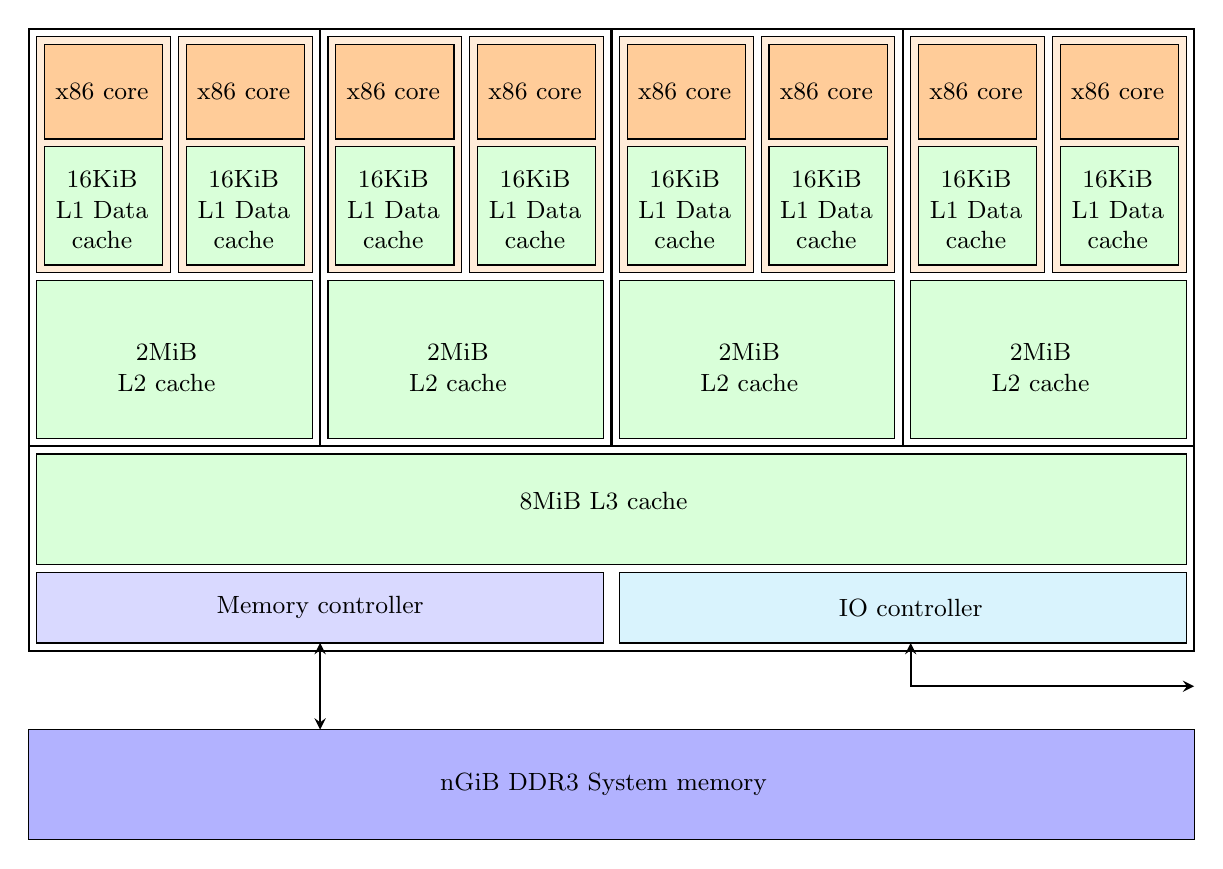
\begin{tikzpicture}[>=stealth]
\draw[thick] (0,0) rectangle ++(14.8, -2.6);
\foreach \x in {0,3.7,7.4,11.1}
{
  \draw[thick] (\x,0) rectangle ++(3.7,5.3);
  \draw[fill=green!15] (\x+0.1,0.1) rectangle ++(3.5,2);
  \draw node[text width=2cm,font=\small, align=center] at (\x+1.75 ,1) {2MiB\\L2 cache};
  \foreach \y in {0,1.8}
  {
    \draw[fill=orange!15] (\x+\y+0.1, 2.2) rectangle ++(1.7,3);
    \draw[fill=green!15] (\x+\y+0.2, 2.3) rectangle ++(1.5,1.5);
    \draw node[text width=1.5cm,font=\small, align=center] at (\x+\y+0.2+0.73, 3.0) {16KiB L1 Data cache};

    \draw[fill=orange!40] (\x+\y+0.2, 3.9) rectangle ++(1.5,1.2);
    \draw node[text width=1.2cm,font=\small, align=center] at (\x+\y+0.2+0.73, 4.5) {x86 core};
  }
}
\draw[fill=green!15] (0.1, -1.5) rectangle ++(14.6, 1.4);
\draw node[text width=3cm,font=\small, align=center] at (7.3,-0.7) {8MiB L3 cache};

\draw[fill=blue!15] (0.1, -2.5) rectangle ++(7.2, 0.9);
\draw node[text width=4cm,font=\small, align=center] at (3.7,-2.05) {Memory controller};

\draw[fill=cyan!15] (7.5, -2.5) rectangle ++(7.2, 0.9);
\draw node[text width=4cm,font=\small, align=center] at (7.5+3.7,-2.05) {IO controller};

\draw[fill=blue!30] (0, -5) rectangle ++(14.8, 1.4);
\draw node[text width=5.2cm,font=\small, align=center] at (7.3,-4.3) {nGiB DDR3 System memory};

\draw[thick, <->] (3.7,-2.5) -- (3.7, -3.6);

\draw[thick, <->] (7.5+3.7,-2.5) -- (7.5+3.7, -3.05) -- (14.8, -3.05);

\end{tikzpicture}
    }
  \end{center}
  \caption{Block diagram of hardware architecture of AMD FX--8150 CPU. Device
    has 8 cores packed into 2--core logical modules sharing FPU unit, 2MiB of
    L2 data cache, instruction fetching/decoding units and branch predictor.}
  \label{fig:bulldozerarch}
\end{figure}

Entire processor is presented to the programmer as a single OpenCL
device\footnote{However with \emph{device fission} mechanism introduced in OpenCL 1.2 (and
earlier with extension) it is possible to divide a device into subdevices based on e.g. memory characteristics}
By default, every core is used to perform computations. For each core, one
thread for dispatching work--groups is created what effectively creates thread
of pools pinned to each of the available cores.

\subsubsection{Mapping to OpenCL logical hierarchy}
If not divided into subdevices, each core of Bulldozer CPU is considered one
OpenCL compute unit. Since CPU doesn't have any controllable cache, RAM is used
for all kinds of OpenCL memories. However, special measures are taken, to ensure
that private memory of work--items and local memory of work--groups is
laid in a way that is optimal for cache locality.
\subsubsection{Execution model}
\begin{figure}[htb]
  \begin{center}
    
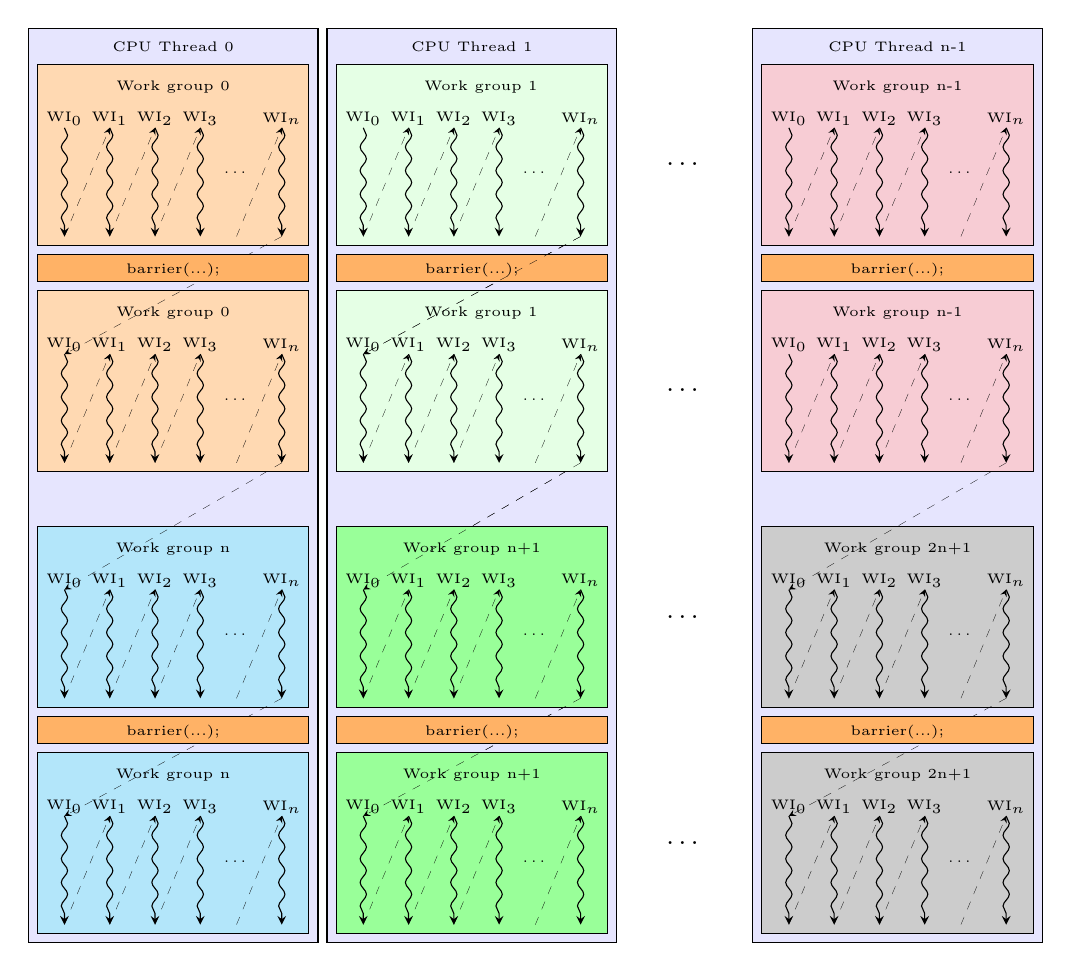
\begin{tikzpicture}[ scale=1.15,
  >=stealth,
  snaky/.style={->,decorate,decoration={name=snake,amplitude=.4mm,segment length=3mm,post length=0.5mm}},
  dashy/.style={->,dashed,ultra thin}
]
\usetikzlibrary{scopes}
\usetikzlibrary{decorations,snakes}

\foreach \x/\xtext in {0/0,3.3/1, 8/n-1}
{
  \draw[fill=purple!5!blue!10] (\x,10) rectangle ++(3.2,-10.1);
  \draw[font=\tiny] node at (\x+3.2/2, 9.8) {CPU Thread \xtext};
}

\def\wavylines#1#2{
\begin{scope}[xshift=#1,yshift=#2]


\draw node [font=\tiny] {WI$_0$};
\draw [snaky] (0,-0.1) -- ++(0,-1.2);

\foreach \x in {1,2,3}
{
  \draw node [font=\tiny] at (0.5*\x, 0) {WI$_\x$};
  \draw [dashy] ( \x*0.5 - 0.5, -1.3) -- ++(0.5,1.2);
  \draw [snaky] ( \x*0.5, -0.1) -- ++(0,-1.2);
}
\draw[font=\tiny] node at (1.9,-0.6) {\ldots};
\draw node at (2.4,0) [font=\tiny] {WI$_n$};
\draw [snaky] (2.4,-0.1) -- ++(0,-1.2);
\draw [dashy] (1.9,-1.3) -- ++(0.5,1.2); 

\end{scope}
} %wavylines

%CPU thread 0

% Work group 0
\draw[fill=orange!30] (0.1,9.6) rectangle ++(3,-2.0);
\draw[font=\tiny] node at (3.2/2, 9.35) {Work group 0};
\wavylines{0.4cm}{9.0cm};

\draw[fill=orange!30] (0.1,7.1) rectangle ++(3,-2.0);
\draw[font=\tiny] node at (3.2/2, 6.85) {Work group 0};
\wavylines{0.4cm}{6.5cm};

\draw[dashy] (2.8,7.7) -- (0.4,6.4);

\draw[fill=orange!60] (0.1,7.5) rectangle ++(3,-0.3);
\draw[font=\tiny] node at (1.6, 7.33) {barrier(...);};

% Work group 1
\draw[fill=cyan!30] (0.1,4.5) rectangle ++(3,-2.0);%CPU thread 1

% Work group 0
\draw[fill=green!10] (3.4,9.6) rectangle ++(3,-2.0);
\draw[font=\tiny] node at (3.4+3.2/2, 9.35) {Work group 1};
\wavylines{3.7cm}{9.0cm};

\draw[fill=green!10] (3.4,7.1) rectangle ++(3,-2.0);
\draw[font=\tiny] node at (3.4 + 3.2/2, 6.85) {Work group 1};
\wavylines{3.7cm}{6.5cm};

\draw[dashy] (3.3 + 2.8,7.7) -- (3.7,6.4);

\draw[fill=orange!60] (3.4,7.5) rectangle ++(3,-0.3);
\draw[font=\tiny] node at (3.3+1.6, 7.33) {barrier(...);};

% Work group 1
\draw[fill=green!40] (3.4,4.5) rectangle ++(3,-2.0);
\draw[font=\tiny] node at (3.3+3.2/2, 4.25) {Work group n+1};
\wavylines{3.7cm}{3.9cm};

\draw[dashy] (3.3+2.8,5.2) -- (3.3+0.4,3.8);

\draw[fill=green!40] (3.3+0.1,2.0) rectangle ++(3,-2.0);
\draw[font=\tiny] node at (3.3+3.2/2, 1.75) {Work group n+1};
\wavylines{3.7cm}{1.4cm};

\draw[dashy] (3.3+2.8,2.6) -- (3.3+0.4,1.3);

\draw[fill=orange!60] (3.3+0.1,2.4) rectangle ++(3,-0.3);
\draw[font=\tiny] node at (3.3+1.6, 2.23) {barrier(...);};
\draw[font=\tiny] node at (3.2/2, 4.25) {Work group n};
\wavylines{0.4cm}{3.9cm};

\draw[dashy] (2.8,5.2) -- (0.4,3.8);

\draw[fill=cyan!30] (0.1,2.0) rectangle ++(3,-2.0);
\draw[font=\tiny] node at (3.2/2, 1.75) {Work group n};
\wavylines{0.4cm}{1.4cm};

\draw[dashy] (2.8,2.6) -- (0.4,1.3);

\draw[fill=orange!60] (0.1,2.4) rectangle ++(3,-0.3);
\draw[font=\tiny] node at (1.6, 2.23) {barrier(...);};

%CPU thread 1

% Work group 0
\draw[fill=green!10] (3.4,9.6) rectangle ++(3,-2.0);
\draw[font=\tiny] node at (3.4+3.2/2, 9.35) {Work group 1};
\wavylines{3.7cm}{9.0cm};

\draw[fill=green!10] (3.4,7.1) rectangle ++(3,-2.0);
\draw[font=\tiny] node at (3.4 + 3.2/2, 6.85) {Work group 1};
\wavylines{3.7cm}{6.5cm};

\draw[dashy] (3.3 + 2.8,7.7) -- (3.7,6.4);

\draw[fill=orange!60] (3.4,7.5) rectangle ++(3,-0.3);
\draw[font=\tiny] node at (3.3+1.6, 7.33) {barrier(...);};

% Work group 1
\draw[fill=green!40] (3.4,4.5) rectangle ++(3,-2.0);
\draw[font=\tiny] node at (3.3+3.2/2, 4.25) {Work group n+1};
\wavylines{3.7cm}{3.9cm};

\draw[dashy] (3.3+2.8,5.2) -- (3.3+0.4,3.8);

\draw[fill=green!40] (3.3+0.1,2.0) rectangle ++(3,-2.0);
\draw[font=\tiny] node at (3.3+3.2/2, 1.75) {Work group n+1};
\wavylines{3.7cm}{1.4cm};

\draw[dashy] (3.3+2.8,2.6) -- (3.3+0.4,1.3);

\draw[fill=orange!60] (3.3+0.1,2.4) rectangle ++(3,-0.3);
\draw[font=\tiny] node at (3.3+1.6, 2.23) {barrier(...);};

\draw node at (7.25,8.5) {\ldots};
\draw node at (7.25,6) {\ldots};
\draw node at (7.25,3.5) {\ldots};
\draw node at (7.25,1.0) {\ldots};

%CPU thread n-1

% Work group 0
\draw[fill=blue!15!red!20] (8.1,9.6) rectangle ++(3,-2.0);
\draw[font=\tiny] node at (8+3.2/2, 9.35) {Work group n-1};
\wavylines{8.4cm}{9.0cm};

\draw[fill=blue!15!red!20] (8.1,7.1) rectangle ++(3,-2.0);
\draw[font=\tiny] node at (8 + 3.2/2, 6.85) {Work group n-1};
\wavylines{8.4cm}{6.5cm};

\draw[dashy] (3.3 + 2.8,7.7) -- (3.7,6.4);

\draw[fill=orange!60] (8.1,7.5) rectangle ++(3,-0.3);
\draw[font=\tiny] node at (8+1.6, 7.33) {barrier(...);};

% Work group 1
\draw[fill=gray!40] (8.1,4.5) rectangle ++(3,-2.0);
\draw[font=\tiny] node at (8+3.2/2, 4.25) {Work group 2n+1};
\wavylines{8.4cm}{3.9cm};

\draw[dashy] (8+2.8,5.2) -- (8+0.4,3.8);

\draw[fill=gray!40] (8+0.1,2.0) rectangle ++(3,-2.0);
\draw[font=\tiny] node at (8+3.2/2, 1.75) {Work group 2n+1};
\wavylines{8.4cm}{1.4cm};

\draw[dashy] (8+2.8,2.6) -- (8+0.4,1.3);

\draw[fill=orange!60] (8+0.1,2.4) rectangle ++(3,-0.3);
\draw[font=\tiny] node at (8+1.6, 2.23) {barrier(...);};

\end{tikzpicture}

  \end{center}
  \caption{Execution model of OpenCL on AMD FX--8150 CPU.}
  \label{fig:clbullexec}
\end{figure}

Each core of the CPU executes work--groups assigned to it one after another.
Within each work--group, each work--item is executed serially until barrier
operation is reached or kernel is finished. When barriers are reached,
work--item execution is suspended, its local state is saved through
\texttt{setjmp} system call to be later restored with \texttt{longjmp}.
Execution then moves to the next work--item within the work--group.

AMD OpenCL
runtime provides modified version of \texttt{setjmp} and \texttt{longjmp} syscalls
that work better with CPU branch predictor and maintain program stack alignment.
This approach is faster than system--level thread preemption because creating
system threads is much more expensive than aforementioned calls.

Within each work--group vector operations from SSE\footnote{Streaming SIMD
Extension} and AVX\footnote{Advanced Vector Extension} extensions are heavily
used to obtain instruction--level parallelism on vector types offered by OpenCL
language specification.

Worth mentioning is the fact, that main program code is executed on the same
processor as OpenCL kernels. Heavy computation in the host code of the application
may severely decrease performance of OpenCL computations.

\subsection{OpenCL on NVIDIA GTX580}

NVIDA GeForce GTX 580 is the most advanced graphic card in GeForce series 500 lineup.
It's a consumer graphics card aimed at users with highest performance needs.
GTX 580 is based on architecture called \emph{Fermi} and will be presented based on
\cite[p59]{gaster2012heterogeneous} and \cite{nvidiafermi}.

\subsubsection{Architecture}
GTX 580 contains 16 Compute Units called \emph{Symmetric Multiprocessors} (SMs).
Each SM contains the following elements (for graphical diagram see
\autoref{fig:fermism}):

\begin{description}
  \item[32 \emph{CUDA Cores}] \hfill \\
    Compute units containing ALU\footnote{Arithmetic Logic Unit}
    for integer arithmetic and FPU\footnote{Floating Point unit} for floating point
    operations conforming to IEEE~754--2008 standard. It also supports multiply--add
    and fused multiply--add operations.
  \item[16 load/store units] \hfill \\
    These units calculate addresses for memory access. They provide access to
    data for 16 threads per clock cycle.
  \item[4 SFUs] \hfill \\
    Special Function Units for execution of transcendental instructions
    like sine, cosine, reciprocal and square root
  \item[2 Warp Schedulers] \hfill \\
    Thread scheduling units that choose 2 packs of 16 threads for concurrent
    execution.
  \item[Register file] \hfill \\
    Area of very fast memory, 128KiB in size\footnote{or $2^{15}$ 32-bit elements}
  \item[Shared memory/L1 cache] \hfill \\
    64 KiB of fast memory configurable as
    16KiB of shared memory and 48KiB of L1 cache or 48KiB of L1 cache and 16 KiB
    of shared memory
\end{description}
\begin{figure}[pb]
  \begin{center}
      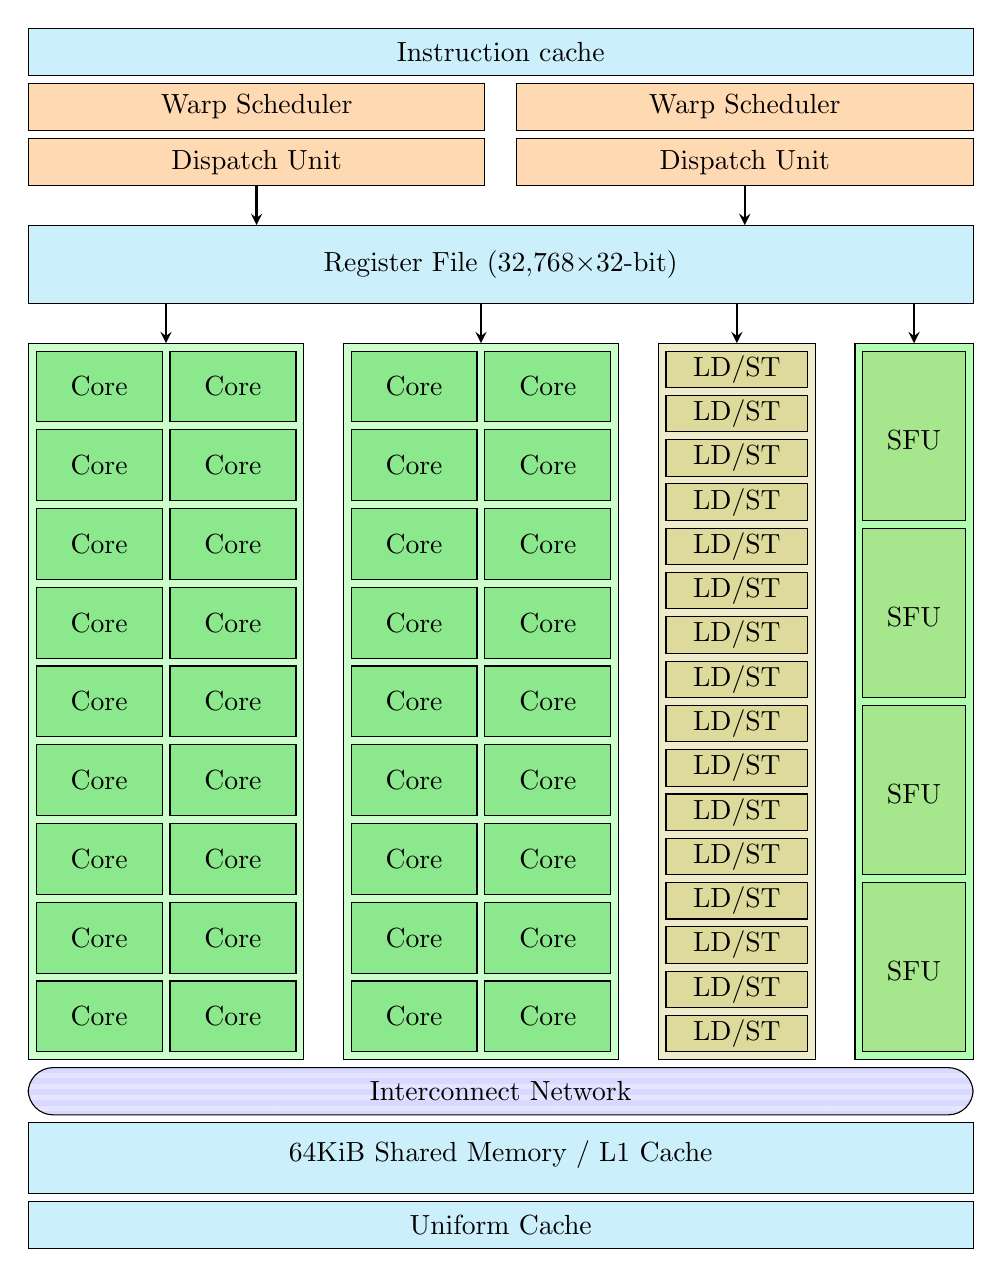
\begin{tikzpicture}[>=stealth]
\usetikzlibrary{patterns}

\draw[fill=cyan!20] (0,0) rectangle ++(12,-0.60);
\draw node at (6,-0.30) {Instruction cache};

\draw[fill=orange!30] (0,-0.7) rectangle ++(5.8,-0.6);
\draw node at (2.9, -1) {Warp Scheduler};

\draw[fill=orange!30] (6.2,-0.7) rectangle ++(5.8,-0.6);
\draw node at (6.2 + 2.9, -1) {Warp Scheduler};

\draw[fill=orange!30] (0,-1.4) rectangle ++(5.8,-0.6);
\draw node at (2.9, -1.7) {Dispatch Unit};

\draw[fill=orange!30] (6.2,-1.4) rectangle ++(5.8,-0.6);
\draw node at (6.2 + 2.9, -1.7) {Dispatch Unit};

\draw[->, thick] (2.9,-2) -- (2.9,-2.5);
\draw[->, thick] (6.2+2.9,-2) -- (6.2+2.9,-2.5);

\draw[fill=cyan!20] (0,-2.5) rectangle ++(12,-1);
\draw node at (6, -2.5-0.5) {Register File (32,768$\times$32-bit)};

\draw[->,thick] (1.75,-3.5) -- ++(0,-0.5);
\draw[->,thick] (5.75,-3.5) -- ++(0,-0.5);

\foreach \x in {0,4}
{
  \draw[fill=green!20] (\x, -4) rectangle (\x+3.5, -13.1);
  \foreach \j in {0,...,8}
  {
    \foreach \k in {0 ,1.7}
    {
      \draw[fill=green!80!black!45] (\x+0.1+\k, -4 - \j*1 -0.1) rectangle ++(1.6,-0.9);
      \draw node at (\x+0.1+\k+0.8, -4 - \j*1 -0.1-0.45) {Core};
    }
  }
}

\draw[->,thick] (9,-3.5) -- ++(0,-0.5);
\draw [fill=olive!15] (8.0,-4) rectangle (10,-13.1);
\foreach \x in {0,...,15}
{
  \draw [fill=olive!30] (8.1, -4.1 - 9.0/16 * \x) rectangle ++(1.8, -9.0/16.0+0.1);
  \draw node at (8.1 + 0.9, -4.1 - 9.0/16 * \x  - 9.0/16.0/2+0.1/2) {LD/ST};
}

\draw[fill=green!30] (10.5, -4) rectangle (12,-13.1);
\draw[->,thick] (10.5 + 0.75,-3.5) -- ++(0,-0.5);
\foreach \x in {0,...,3}
{
  \draw[fill=green!60!brown!50] (10.6, -4.1 - 9.0/4*\x) rectangle ++(1.3, -9.0/4+0.1);
  \draw node at  (10.6 + 1.3/2, -4.1 - 9.0/4*\x - 9.0/4/2) {SFU};
}

\draw[pattern=horizontal lines light blue,rounded corners=9pt] (0,-13.2) rectangle ++(12,-0.60);
\draw node at (6,-13.50) {Interconnect Network};

\draw[fill=cyan!20] (0,-13.9) rectangle ++(12,-0.90);
\draw node at (6,-14.30) {64KiB Shared Memory / L1 Cache};

\draw[fill=cyan!20] (0,-14.9) rectangle ++(12,-0.60);
\draw node at (6,-15.20) {Uniform Cache};

\end{tikzpicture}
  \end{center}
  \caption{Hihg--level overview of elements forming Fermi SM}
  \label{fig:fermism}
\end{figure}

These 16 SMs are accompanied by following units in the chip
\begin{itemize}
  \item 6 64-bit GDDR5 memory units forming 384-bit
memory interface that supports up to 6GiB of DRAM, 768KiB of L2 cache
  \item GigaThread engine for distributing blocks\footnote{or work--groups in OpenCL nomenclature}
  among SMs
  \item host communication interface\footnote{PCI-Express bus}.
\end{itemize}

\subsubsection{Mapping to OpenCL logical hierarchy}

Single Fermi GPU is visible as one OpenCL device. SMs are equivalent to Compute
Units, and CUDA cores are mapped to Processing Elements. GDDR5 DRAM implements
global memory, per--SM shared memory is used for OpenCL local memory,
register file is used for private memory, and constant memory is located on
dedicated DRAM units with separate cache. Images are implemented using texture
memory, the same one that is used for graphics processing.

\subsubsection{Execution model}

When kernel is scheduled for execution on Fermi GPU it's enqueued in GigaThread
engine that distributes work--groups among available SMs.

When work--group arrives at the SM, it's further divided into units of 32 threads
called \emph{warps}. At one cycle, two warps are selected that go to each
Warp Scheduler. Both Warp Schedulers issue one instruction from each warp to
one of following parts of SM:
\begin{itemize}
  \item 16 CUDA cores\footnote{In these case, these 16 threads form a half-warp}
  \item 16 Load/Store units
  \item 4 SFUs
\end{itemize}

Most of instructions in both warps can be issued independently, so this
dual--scheduling technique helps in achieving peak hardware utilization.

\subsubsection{Pitfalls of OpenCL programming on GPU}

Execution model described in previous section clearly prefers execution of the same instruction
on many threads. NVIDIA call this model SIMT or ,,Single Instruction Multiple
Thread``. When just one thread diverges in code path through e.g. \texttt{if}
statement, every possible code path must be executed for each thread in a half--warp.
That's why kernels with divergent code flows should be avoided.

Another problem is usage of registers. Since execution isn't stack--based like
in x86 CPUs, every local variable must go to Register File on SM that is rather
small. When too many registers are used, either less blocks will be able to
be computed at the same time, or register spilling mechanism that uses orders
of magnitude slower global memory as a backup location for overflowing variables
will kick in. Both of these possibilities may significantly reduce performance.

As mentioned before, execution of threads on GPU isn't stack based. All function
calls in kernels are inlined. Therefore, algorithms that rely on recursion with
arbitrary depth may be very hard to implement.
